
	\begin{frame}{3.7 링크보}
	\textbf{3.7.1 일반사항}
	
	\begin{enumerate}
		\item[(1)] 이 절은 편심가새골조의 구성요소인 링크보에 적용한다. 
		\item[(2)] 링크보는 가새골조를 구성하는 여러 부재의 작용선이 단일 지점에서 교차하지 않고, 작용점 간의 거리(편심거리 $e$)가 접합부에 연결된 가장 작은 부재의 폭을 초과해야 한다. 
	\end{enumerate}
		
	\begin{block}{링크보 거동의 분류}
		\begin{itemize}
			\item $l_b \geq 2.6M_{CE}/V_{CE}$: 링크보 부재는 휨지배거동 $\rightarrow$ 3.7절 링크보
			\item $l_b < 1.6M_{CE}/V_{CE}$: 링크보 부재는 전단지배거동 $\rightarrow$ 3.7절 링크링크보요소
			\item Otherwise: 링크보 부재는 휨--전단지배 $\rightarrow$ 링크보의 길이에 따라 선형링크보간
		\end{itemize}
	\end{block}

	\textbf{3.7.2 링크보의 강성}
	
	3.7.2.1 선형동적절차
	
	\begin{enumerate}
		\item[(1)] 링크보의 부재력--변형 모델은 전단변형과 휨변형을 포함하여야 한다. 
		\item[(2)] 린크보의 탄성구간 강성 $K_e$는 아래 식을 사용하여 산정할 수 있다. 
		\[K_e = \frac{12EI}{e^3(1+\eta)}\]
	\end{enumerate}		
	
	\end{frame}


	\begin{frame}{3.7 링크보}

	\textbf{3.7.2 링크보의 강성}
	
	3.7.2.2 비선형정적절차
	
	\begin{enumerate}
		\item[(1)] 링크보 부재의 탄성구간 강성은 3.7.2.1에 따라 산정한다.
		\item[(2)] 링크보 부재의 비선형 부재력--변형 모델링은 실험이나 정밀해석을 통해 얻어진 관계를 사용하거나, 그림 1-1과 같은 일반화된 부재력--변형 관계로부터 3.1.2.2절을 다음을 따른다.
		\item[(3)] 링크보의 항복회전각은 아래 식을 사용하여 산정한다. 
		\[\theta_y \equiv \gamma_y = \frac{Q_{CE}}{K_e e}\] 
		\noindent 여기서 $Q_{CE}$는 3.7.3절에 따라 산정한 링크보요소의 예상부재강도이고, $K_e$는 링크보요소의 탄성구간 강성이다. 
		\begin{figure}
			\centering
			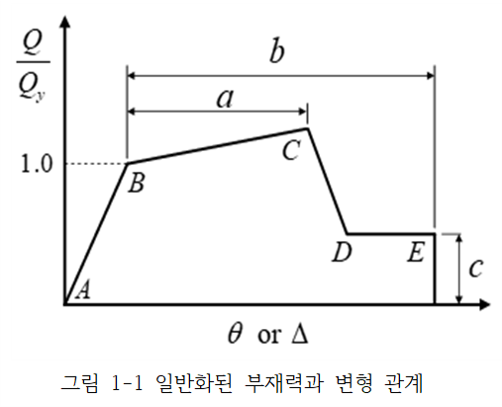
\includegraphics[width=0.5\textwidth]{image01}
		\end{figure}
	\end{enumerate}
	\end{frame}
	
	\begin{frame}{3.7 링크보}

	\textbf{3.7.2 링크보의 강성}
	
	3.7.2.3 비선형동적절차
	
	링크보 부재의 이력거동 모델링은 실험이나 정밀해석을 통해 얻어진 관계를 사용할 수 있다. 
	\end{frame}	
	
	
	\begin{frame}
		\begin{figure}
			\centering
			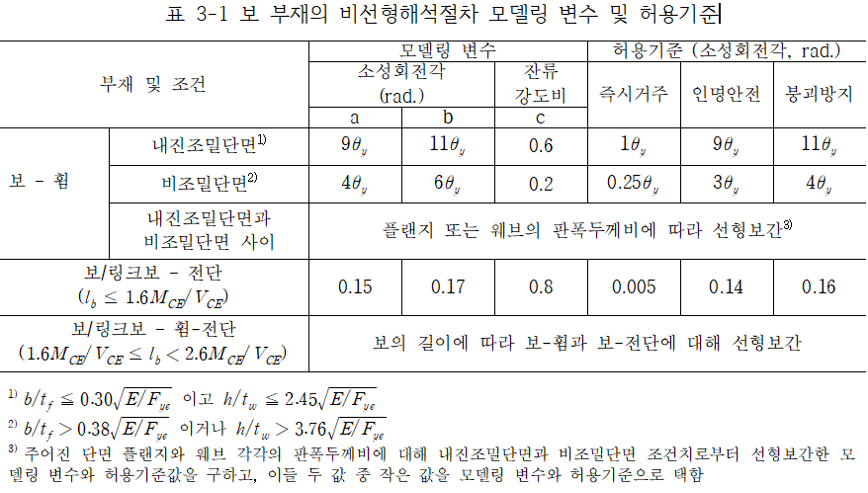
\includegraphics[width=.99\textwidth]{table01}
		\end{figure}
	\end{frame}


	\begin{frame}{3.7 링크보}

	\textbf{3.7.3 링크보의 강도}
	
	3.7.3.7 선형동적절차
	
	\begin{enumerate}
		\item[(1)] 링크보의 예상부재강도 $Q_{CE}$는 예상전단강도 $V_{CE}$ 혹은 예상휨강도 $M_{CE}$에 의해 지배된다. 
		\item[(2)] 전단항복에 의해 지배될 경우, 링크보의 예상부재강도 $Q_{CE}(=Q_y=V_{CE})$는 아래 식을 통해 산정한다.  
			\[V_{CE} = V_{ye} = \begin{dcases}0.6F_{ye}A_s & \frac{\vert P\vert}{P_{ye}} \leq 0.2 \\0.6F_{ye}A_s\sqrt{1 - \Big(\frac{\vert P\vert}{P_{ye}}\Big)^2} & \frac{\vert P\vert}{P_{ye}} > 0.2\end{dcases}\]
		\item[(3)] 휨항복의 경우 링크보의 예상부재강도 $Q_{CE}(=Q_y=V)$는 예상휨강도에서 소요전단강도로 변환하여 아래 식을 통해 산정한다.
			\[V = 2M_{CE}/e\] 
	\end{enumerate}
	\end{frame}	


	\begin{frame}{3.7 링크보}

	\textbf{3.7.3 링크보의 강도}
	
	3.7.3.2 비선형정적 및 동적절차
	
	\begin{enumerate}
		\item[(1)] 비선형정적절차의 경우 실험이나 정밀해석을 통해 얻어진 관계를 사용할 수 있으며, 3.7.2.2절의 비선형 부재력--변형 관계를 결정한다. 
		\item[(2)] 비선형동적절차의 이력거동 모델링은 실험이나 정밀해석을 통해 얻어진 관계를 사용할 수 있으며, 포락곡선으로는 표 3-1에 사용된 모델을 적용할 수 있다. 
	\end{enumerate}
	\end{frame}	
	

	\begin{frame}{3.7 링크보}

	\textbf{3.7.4 링크보의 허용기준}
	
	3.2.4.1 일반사항
	
	링크보는 전단과 휨에 대해 변형지배거동으로 분류한다. 
	
	3.2.4.2	선형동적절차
	
	\begin{enumerate}
		\item[(1)] 링크보의 휨 및 전단거동에 대한 $m$계수는 표 3-2를 따른다. 
		\item[(2)] 링크보의 상세는 $\ulcorner$건축물 강구조 설계기준$\lrcorner$의 요구사항을 만족하여야 한다. 
		\item[(3)] 편심가새골조 내의 링크보에 연결된 가새, 기둥 및 기타 요소는 링크보의 예상휨강도 $M_{CE}$와 예상전단강도 $V_{CE}$ 중 작은 값의 1.25배가 되도록 설계한다. 
		\item[(4)] 압축강도비 $P_{UF}/P_{ye}$가 0.6을 초과하는 링크보는 모든 조건에서 탄성범위 이내에 있어야 하며 $m$계수는 1.0을 적용한다.  
	\end{enumerate}
	
	3.2.4.2 비선형 정적 및 동적절차	
	
	\begin{enumerate}
		\item[(1)] 링크보의 변형한계는 표 3-2, 3-6과 3-7를 따른다. 
		\item[(2)] 압축강도비 $P_{UF}/P_{ye}$가 0.6을 초과하는 링크보는 모든 조건에서 탄성범위 이내에 있어야 하며 허용소성회전각은 0을 적용한다. 
	\end{enumerate}
	\end{frame}	

	\begin{frame}
		\begin{figure}
			\centering
			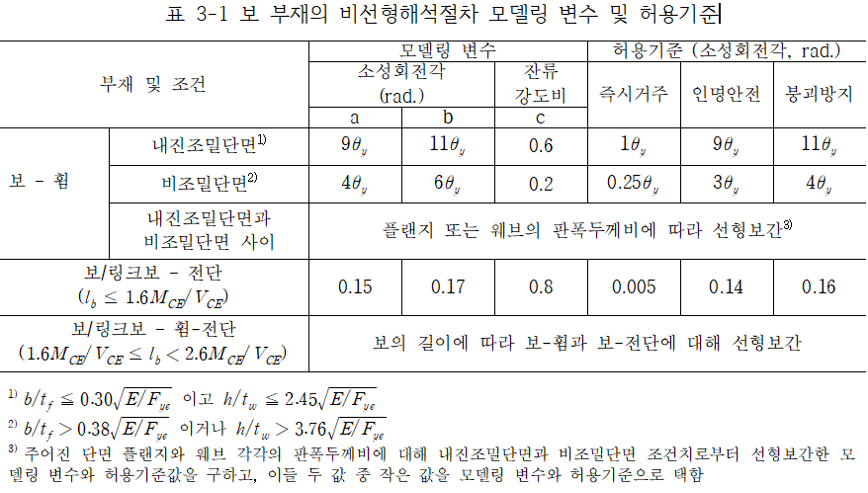
\includegraphics[width=.99\textwidth]{table01}
		\end{figure}
	\end{frame}
	
	\begin{frame}
		\begin{figure}
			\centering
			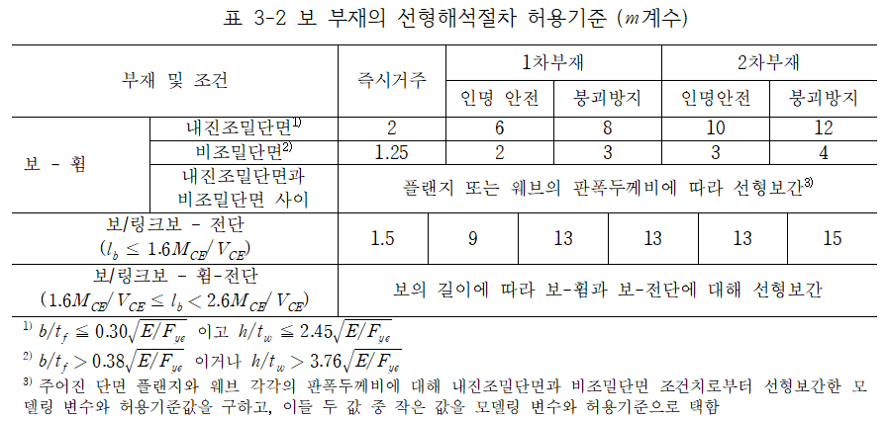
\includegraphics[width=.99\textwidth]{table02}
		\end{figure}
	\end{frame}	
	